% Generated by python3 -m squares.paper.figures; do not edit.
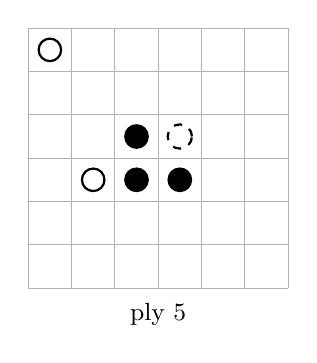
\begin{tikzpicture}[scale=0.55]
  \draw[gray!60] (0,0) grid (6,-6);
  \foreach \r/\c in {2/2, 3/2, 3/3}
    \filldraw[fill=black,thick] (\c+0.5,-\r-0.5) circle (0.26);
  \foreach \r/\c in {0/0, 3/1}
    \filldraw[fill=white,thick] (\c+0.5,-\r-0.5) circle (0.26);
  \draw[thick,dashed] (3.5,-2.5) circle (0.28);
  \node at (3,-6.6) {\small ply 5};
\end{tikzpicture}
\hspace{1em}
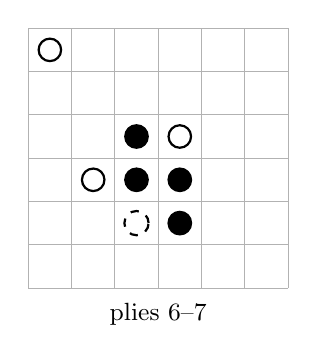
\begin{tikzpicture}[scale=0.55]
  \draw[gray!60] (0,0) grid (6,-6);
  \foreach \r/\c in {2/2, 3/2, 3/3, 4/3}
    \filldraw[fill=black,thick] (\c+0.5,-\r-0.5) circle (0.26);
  \foreach \r/\c in {0/0, 3/1, 2/3}
    \filldraw[fill=white,thick] (\c+0.5,-\r-0.5) circle (0.26);
  \draw[thick,dashed] (2.5,-4.5) circle (0.28);
  \node at (3,-6.6) {\small plies 6--7};
\end{tikzpicture}
\hspace{1em}
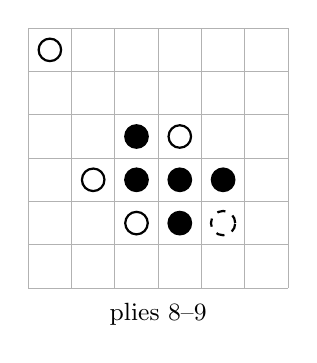
\begin{tikzpicture}[scale=0.55]
  \draw[gray!60] (0,0) grid (6,-6);
  \foreach \r/\c in {2/2, 3/2, 3/3, 4/3, 3/4}
    \filldraw[fill=black,thick] (\c+0.5,-\r-0.5) circle (0.26);
  \foreach \r/\c in {0/0, 3/1, 2/3, 4/2}
    \filldraw[fill=white,thick] (\c+0.5,-\r-0.5) circle (0.26);
  \draw[thick,dashed] (4.5,-4.5) circle (0.28);
  \node at (3,-6.6) {\small plies 8--9};
\end{tikzpicture}
